\documentclass[a4paper]{article}    % define document layout
%\documentclass[draft]{article}     % use draft option in packages
%-----------------------------
% preamble
%-----------------------------
\usepackage[sumlimits,]{amsmath}    % math equations and formulas
\usepackage[utf8]{inputenc}         % use UTF-8 encoding
\usepackage[english]{babel}         % use English language
\usepackage{graphicx}              % insert images
%\usepackage[draft]{graphicx}        % do not render figures
\usepackage{subcaption}             % multiple images in one figure
\usepackage{hyperref}               % hyperlinks
\usepackage{float}                  % floating objects (figures, tables)
\usepackage{geometry}               % page size and margins
\geometry{a4paper, margin=1in}      % margins
\usepackage{ragged2e}               % text alignment
\usepackage[table]{xcolor}          % change cell color in tables
%\usepackage{multirow}               % merge rows in table
%\usepackage[thinc]{esdiff}          % macros for derivatives

\graphicspath{                      % path for figures
    {../figures/} 
}

%-----------------------------
% body
%-----------------------------
\begin{document}

\begin{figure}
    \centering
    % UNICAMP logo
    \begin{subfigure}{0.45\textwidth}
        \centering
        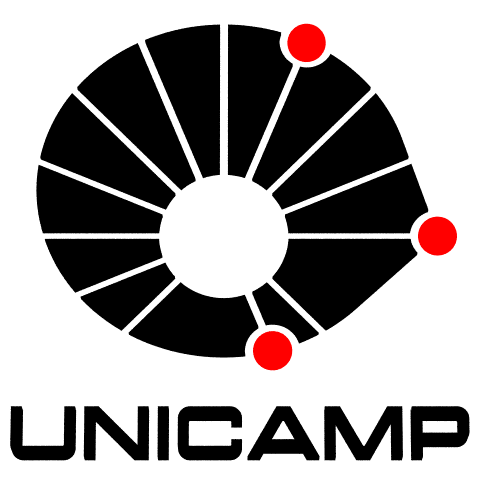
\includegraphics[width=1.5cm]{unicamp}
%        \label{fig:unicamp}
    \end{subfigure}
    \hfill
    % FEEC logo
    \begin{subfigure}{0.45\textwidth}
        \centering
        
\includegraphics[width=1.5cm]{feec}
%        \label{fig:feec}
    \end{subfigure}
\end{figure}

\title{
    \vspace{5cm}
    IA353A - Neural Networks\\
    EC1
    \vspace{1cm}
}
\author{
    Rafael Claro Ito\\
    (R.A.: 118430)
    \vspace{11cm}
}
%R.A.: 118430
%ito.rafael@gmail.com
\date{May 2020}
\maketitle
\newpage

%=================================================
\section*{Question 1}
%=================================================

\newpage

%=================================================
\section*{Question 2}
%=================================================

\[\|Ax-b\|_{P}^{2}+\|x-x_{0}\|_{Q}^{2}\]
%------------------------
\paragraph{Since we are searching for $x$ that minimizes the previous expression, we will calculate the derivative with relation to $x$ and set it equal to zero:}
    \[\frac{d}{dx} (\|Ax-b\|_{P}^{2}+\|x-x_{0}\|_{Q}^{2}) = 0\]
%------------------------
\paragraph{Property used: $\|x\|_{Q}^{2} = x^{T}Qx$}
    \[\frac{d}{dx} [\overbrace{(Ax-b)^{T} P (Ax-b)}^{\|Ax-b\|_{P}^{2}} + \overbrace{(x-x_0)^T Q (x-x_0)}^{\|x-x_{0}\|_{Q}^{2}}] = 0\]
%------------------------
\paragraph{Property used: $(M + N)^T = M^T + N^T$}
    \[\frac{d}{dx} \{[(Ax)^T-b^T] P (Ax-b) + (x^T-x_0^T) Q (x-x_0)\} = 0\]
%------------------------
\paragraph{Property used: $(MN)^T = N^T M^T$}
    \[\frac{d}{dx} \{[x^TA^T-b^T] P (Ax-b) + (x^T-x_0^T) Q (x-x_0)\} = 0\]
    \[\frac{d}{dx} [(x^TA^TPAx - x^TA^TPb -b^TPAx + b^TPb) + (x^TQx - x^TQx_0 - x_0^TQx + x_0^TQx_0)] = 0\]
%------------------------
\paragraph{Properties used:}
    \begin{itemize}
        \item $\frac{d}{dy}(y^TMy) = M^Ty + My$.
        \item $\frac{d}{dy}(y^TMy) = 2My$, if $M = M^T$ (i.e. $M$ is simetric)
        \item $\frac{d(Ax)}{dx} = A$
        \item $\frac{d(x^TA)}{dx} = A^T$
        \item obs.: $A^TPA$ is simetric, since $(A^TPA)^T = (PA)^T(A^T)^T = A^TP^TA$, but $P^T = P$, since P is simetric. Then $A^TPA = (A^TPA)^T$
    \end{itemize}
\paragraph{Using the previous properties, we have:}
    \[\frac{d}{dx} [(x^TA^TPAx - x^TA^TPb -b^TPAx + b^TPb) + (x^TQx - x^TQx_0 - x_0^TQx + x_0^TQx_0)] = 0\]
    \[[2A^TPAx - (A^TPb)^T - b^TPA + 0] + [2Qx - (Qx_0)^T - x_0^TQ + 0] = 0\]
    \[2A^TPAx - (Pb)^T(A^T)^T - b^TPA + 2Qx - x_0^TQ^T - x_0^TQ = 0\]
    \[2A^TPAx - b^TP^TA - b^TPA + 2Qx - x_0^TQ - x_0^TQ = 0\]
    \[2A^TPAx - b^TPA - b^TPA + 2Qx - x_0^TQ - x_0^TQ = 0\]
    \[2A^TPAx - 2b^TPA + 2Qx - 2x_0^TQ = 0\]
    \[2A^TPAx + 2Qx = 2b^TPA + 2x_0^TQ\]
    \[A^TPAx + Qx = b^TPA + x_0^TQ\]
    \[(A^TPA + Q)^{-1}(A^TPA + Q)x = (A^TPA + Q)^{-1}(b^TPA + x_0^TQ)\]
    \[x = (A^TPA + Q)^{-1}(b^TPA + x_0^TQ)\]
    \[x = (A^TPA + Q)^{-1}(b^TP^TA + x_0^TQ^T)\]
    \[x = (A^TPA + Q)^{-1}[(Pb)^TA + (Qx_0)^T]\]
    \[x = (A^TPA + Q)^{-1}[(A^TPb)^T + (Qx_0)^T]\]
    \[\boxed{x = (A^TPA + Q)^{-1}(A^TPb + Qx_0)^T}\]
%------------------------
%\paragraph{Properties used:}
%    \begin{itemize}
%        \item Since $Q$ is simetric, $(Qx_0)^T = Qx_0$
%        \item Since $P$ is simetric, $(A^TPb)^T = (A^TPb)$
%    \end{itemize}
%\paragraph{Then:}
%    \[x = (A^TPA + Q)^{-1}[(A^TPb)^T + (Qx_0)^T]\]
%    \[x = (A^TPA + Q)^{-1}(A^TPb + Qx_0)\]
%------------------------
\newpage

%=================================================
\section*{Question 3}
%=================================================

%=================================================
\section*{Question 4}
%=================================================

%=================================================
\section*{Question 5}
%=================================================

%=================================================
\section*{Question 6}
%=================================================

\end{document}
